\documentclass{beamer}
\usepackage{graphicx} % Required for inserting images
\usepackage[utf8]{inputenc}
\usepackage{enumitem}

\usetheme{Madrid}
\usecolortheme{default}

\title{Modélisation de l'évolution de la température dans une maison.}
\subtitle{Approche par un automate cellulaire.}
\author{Huet Natanéo \and Hurot Eliott}
\date{2024}
\logo{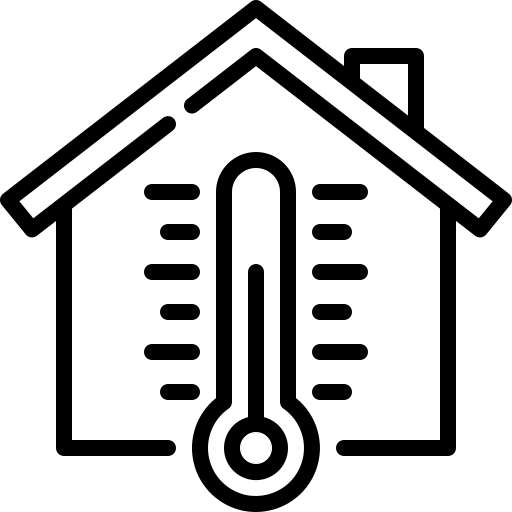
\includegraphics[height=1cm]{room-temperature.png}}

\begin{document}

\frame{\titlepage}

\begin{frame}
    \frametitle{Sommaire}
    \tableofcontents
\end{frame}

\section{Définition d'automate cellulaire}
\begin{frame}
    \frametitle{Définition d'automate cellulaire}

    4-uplet \( ( d, Q, V, \delta) \)
    \begin{itemize}[label=\square]
        \item \(d\) est la dimension;
        \item \(Q\) est l'alphabet;
        \item \(V\) est le voisinage;
        \item \( \delta : Q^{\alpha} \longrightarrow Q \) est la règle de transistion;
    \end{itemize}
\end{frame}

\section{Premier modèle}
\begin{frame}
    \frametitle{Premier modèle}

    \[ 
    \Delta T_{cellule} = \frac{\Delta T_{difference} \times \Delta t} {R_{th} \times C_v} 
    \]

    
    
\end{frame}

\section{Règles de l'automate cellulaire}
\begin{frame}
    \frametitle{Règles de l'automate cellulaire}

\end{frame}

\section{Ajout du chauffage}
\begin{frame}
    \frametitle{Ajout du chauffage}
    
\end{frame}

\end{document}
